\begin{frame}
    \frametitle{GNSS (Global Navigation Satellite System)}
     \note{Página que explica como funciona un GNSS http://gutovnik.com/como_func_sist_gps.html}
     \note{video explicativo: https://youtu.be/U3eX6QKS9kY}
     
     \begin{center}
        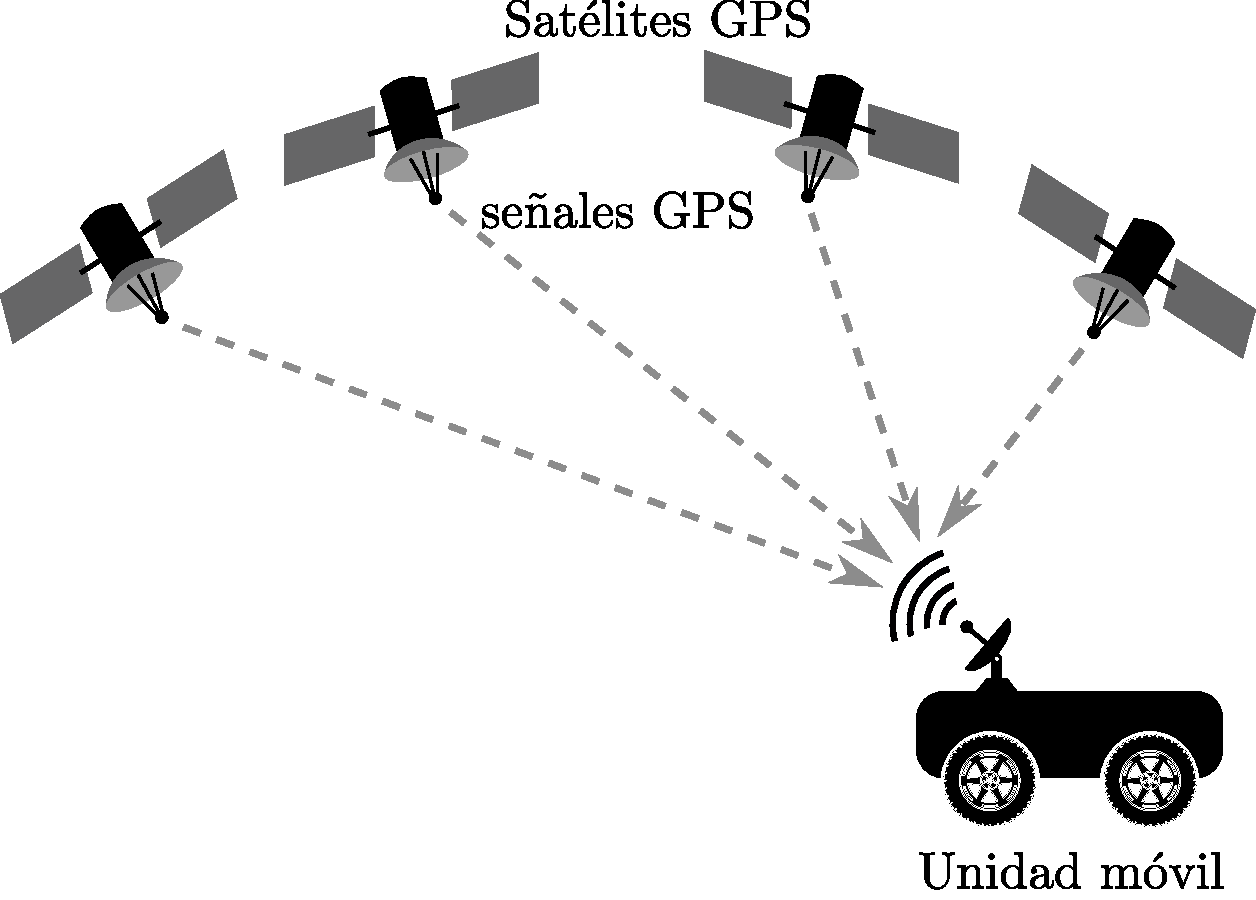
\includegraphics[width=0.3\columnwidth]{gps.pdf}
     \end{center}
    
    \begin{block}{Principio de Funcionamiento}
        Se toma la distancia a cuatro satélites (uno por cada incógnita: latitud, longitud, altitud y offset en tiempo del reloj del receptor) y se estima la pose por triangulación. La distancia a cada satélite se obtiene midiendo el tiempo que tarda en llegar la señal de radio del satélite.
    \end{block}
    
    \note{En el caso del GNSS estamos midiendo una señal de radio, que sabemos que viaja a la velocidad de la luz, alrededor de 300.000 km por segundo.}
    \note{La señal que recibe un receptor de GNSS no es solamente un Código Pseudo Aleatorio con fines de timing. También contiene un mensaje de navegación con información sobre la órbita exacta del satélite}
    \note{Otra manera de manejar los errores inducidos por la atmósfera es comparar la velocidad relativa de dos señales diferentes. Esta medición de doble frecuencia es muy sofisticada y solo es posible en receptores GNSS muy avanzados. Estos son los GNSS-RTK!}
    \note{Los receptores "normales" basados navegación por satélite, comparan una señal pseudoaleatoria que es enviada desde el satélite con una copia interna generada por la misma señal. Puesto que la señal del satélite tarda tiempo en alcanzar al receptor, las dos señales no se alinean correctamente, la copia del satélite se retrasa en referencia a la copia local. Al retrasar progresivamente la copia local, las dos señales se alinearán correctamente en algún momento. Este retraso es el tiempo necesario para que la señal alcance al receptor, y del resultado de esto puede ser calculada la distancia al satélite. La precisión de la medición resultante es generalmente una función de la capacidad  electrónica del receptor para comparar exactamente las dos señales.}
    
    \begin{itemize}
        \item Fuentes de ruido (Retrasos ionosféricos y atmosféricos, Efecto Multitrayectoria, Dilución de la Precisión, reloj del satélite)
        \item Error de posicionamiento métrico ($\sim\SI{2}{\meter}$)
    \end{itemize}
    
    \note{La Dilución de la Precisión (DOP) es una medida de la fortaleza de la geometría de los satélites y está relacionada con la distancia entre los estos y su posición en el cielo. El DOP puede incrementar el efecto del error en la medición de distancia a los satélites.\\
    Un ejemplo de Dilución de la Precisión, si los satélites están en una misma línea (colineales) uno arriba del otro, queda como mal condicionado.}

\end{frame}

\begin{frame}
    \frametitle{Sistema GNSS-RTK (Real-Time Kinematics)}
    \begin{center}
        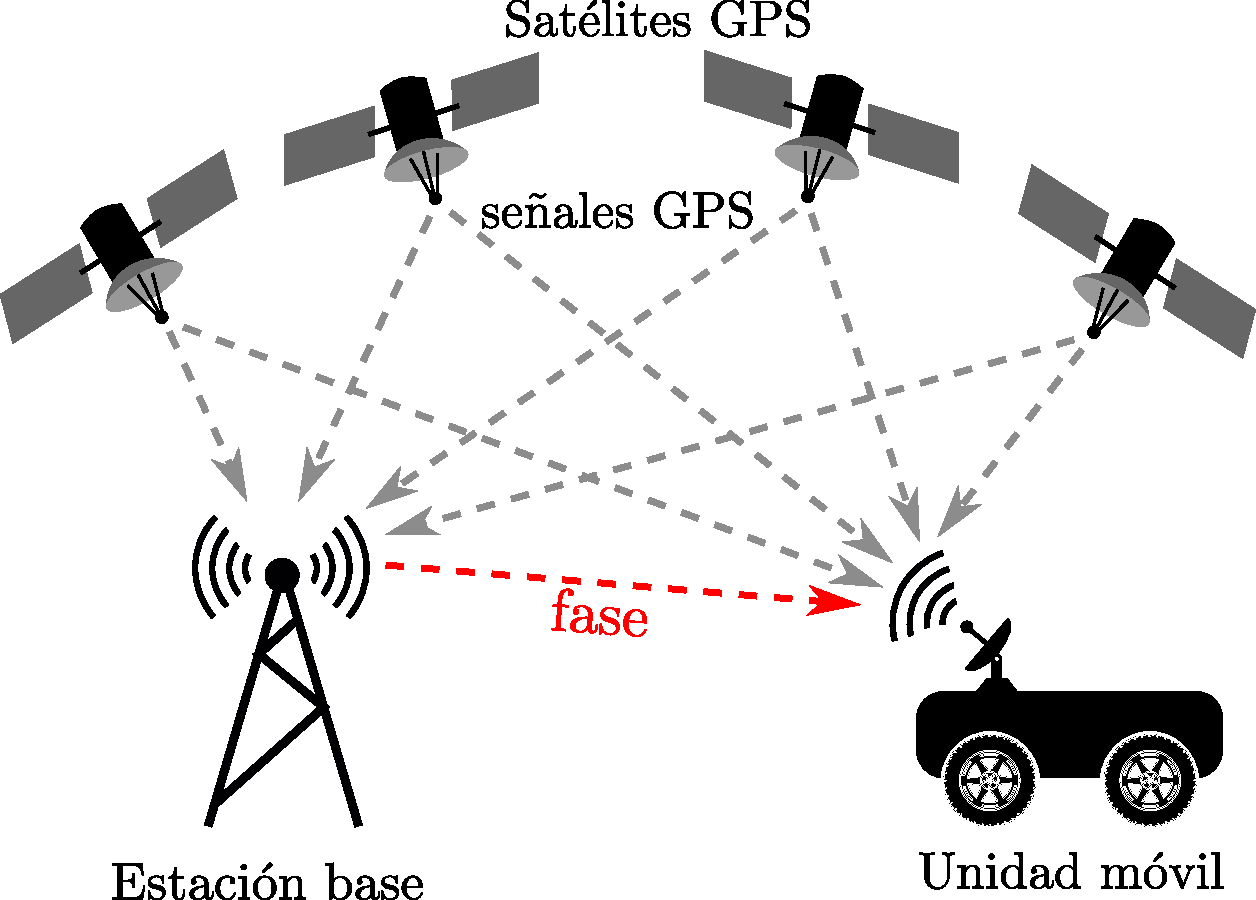
\includegraphics[width=0.3\columnwidth]{gps_rtk_system.pdf}
    \end{center}
    
    \begin{block}{Principio de Funcionamiento}
        \begin{itemize}
            \item Se requieren al menos dos receptores GPS (estación base y unidad móvil). 
            \item La estación base retransmite la fase de la onda portadora de la señal enviada por el satélite \note{no tiene en cuenta los datos enviados por el satélite}
            \item La unidad móvil compara su medición de fase de la señal con la fase recibida de la estación base (\emph{Resolución de Ambig{\"u}edad})
        \end{itemize}
    \end{block}
 
    \begin{itemize}
        \item Error de posicionamiento submétrico ($\sim\SI{0.05}{\meter}$).
        \item Alcance de \SI{10}{\km}
    \end{itemize}

    %
    \note{ RESOLUCIÓN DE AMBIGUEDAD\\
        La sincronización entre la portadora de la señal recibida y la réplica generada en recepción permite obtener una medida de la fase de la portadora. Esta medida de fase puede ser utilizada también para estimar la distancia satélite-receptor. Sin embargo, para ello, es necesario conocer el número entero de ciclos de portadora transcurridos desde que la señal deja el satélite hasta que llega al receptor.\\
        Para realizar la sincronización entre la portadora de la señal y la réplica es necesario tener en cuenta el efecto doppler que se produce debido al movimiento relativo satélite receptor. Por ello, la frecuencia de la réplica ha de ser igual a la frecuencia de la señal transmitida con su desplazamiento doppler corregido. La sincronización se realiza mediante circuitos de enganche en fase (Phase Lock Loop, PLL) o en frecuencia (Frecuency Lock Loop, FLL). Los circuitos PLL o FLL permiten obtener medidas de fase con precisiones del orden de 0.01 ciclos de portadora.\\
        Una vez que el receptor se sincroniza con la portadora y con el código, es decir, se produce el enganche con la señal del satélite, el receptor puede medir la fase de la portadora recibida. Esta medida se obtiene de forma parecida a como se obtiene la medida de pseudodistancia, pues será el desfase que es necesario realizar a la réplica de la portadora para que se sincronice con la portadora recibida. La medida de fase se suele expresar en ciclos de portadora. Por tanto, tal como se ha descrito hasta ahora, la medida de fase será un valor decimal, no entero, indicando la fracción de ciclo de portadora transcurrido en el momento de la recepción de la señal. La distancia entre el satélite y el receptor se puede expresar en número de longitudes de onda y será igual al número entero de ciclos de portadora n transcurridos en el origen desde que la señal salió del satélite hasta que llegó al receptor, más la fracción de ciclo medida (la medida de fase). Por tanto, la medida de fase sirve como estimación de la distancia satélite-receptor pero tiene el problema de que el número entero n es desconocido. A dicho número se le denomina ambigüedad entera de ciclos de portadora. Mientras el receptor permanezca enganchado con la señal el número entero n desconocido permanecerá constante, pues el receptor registra la variación del número entero de ciclos en las propias medidas de fase. La figura 1.7 ilustra esta circunstancia. En el instante t 0 se produce el enganche, obteniéndose la medida phi 0 y siendo desconocido el número de ciclos n. A partir de entonces, el receptor registra la variación de ciclos que se van produciendo y en los instantes sucesivos las medidas de fase phi i estarán formadas por una parte fraccional y una parte entera: la diferencia entre el número de ciclos transcurridos y el número n de la medida inicial. Por tanto, el único valor desconocido es el número entero de ciclos n inicial.}
\end{frame}


\begin{frame}
    \frametitle{Sistema GNSS-PPK (Post Processed Kinematic)}
    \begin{center}
        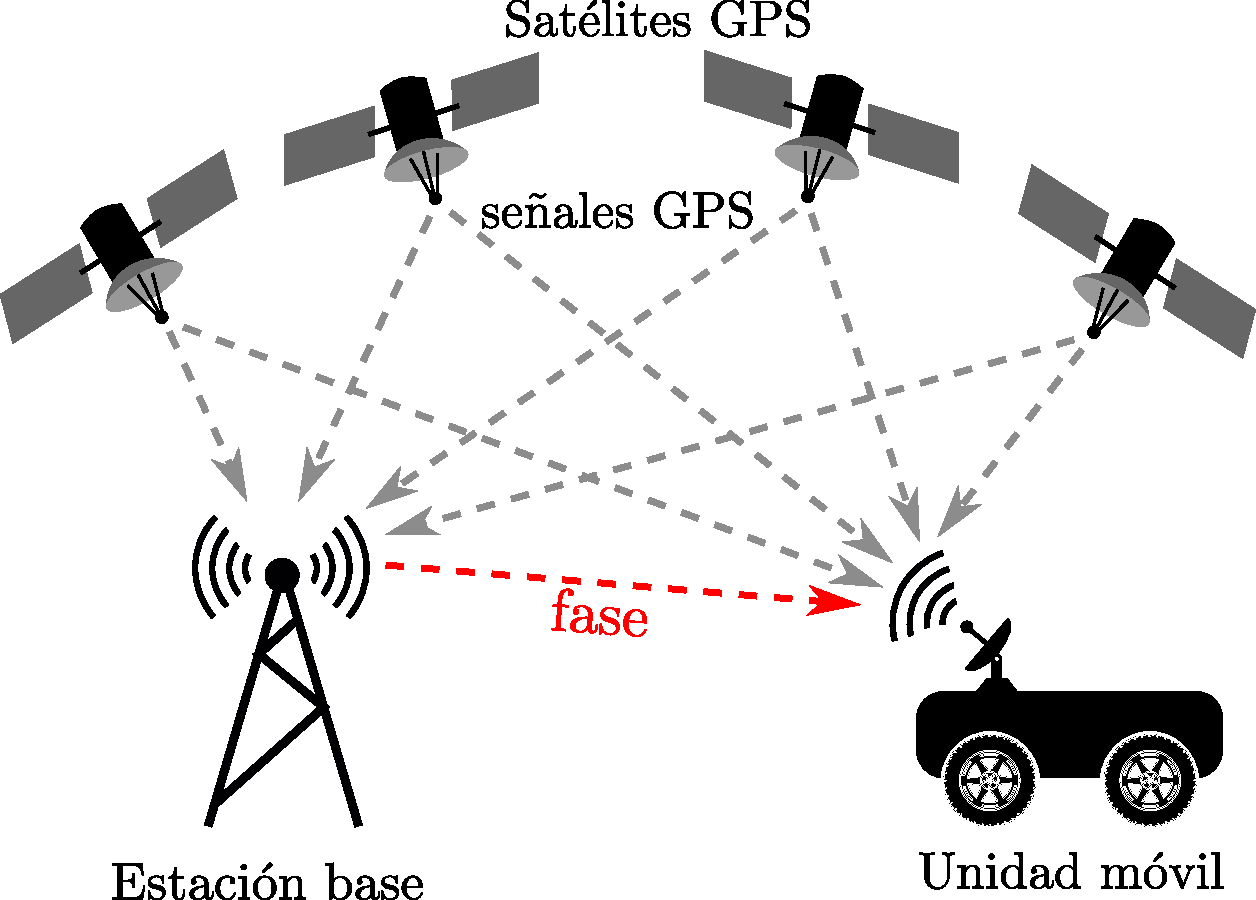
\includegraphics[width=0.3\columnwidth]{gps_rtk_system.pdf}
    \end{center}

    El PPK (Post Processed Kinematic), a diferencia del RTK, realiza un proceso de datos a posteriori (offline).
    En la imagen vemos que, tanto la base como el drone, reciben lecturas de las diferentes constelaciones de satélites. Pero, a diferencia del RTK, no hay un enlace de datos constante entre el drone y la base, ya que ambos registran en una memoria esa información que después del vuelo deberemos descargar, normalmente en archivos con formato RINEX, para postprocesar y obtener nuestra solución.
    
\end{frame}

\begin{frame}
    \frametitle{Sistema GNSS-PPP (Precise Point Positioning)}
    \begin{center}
        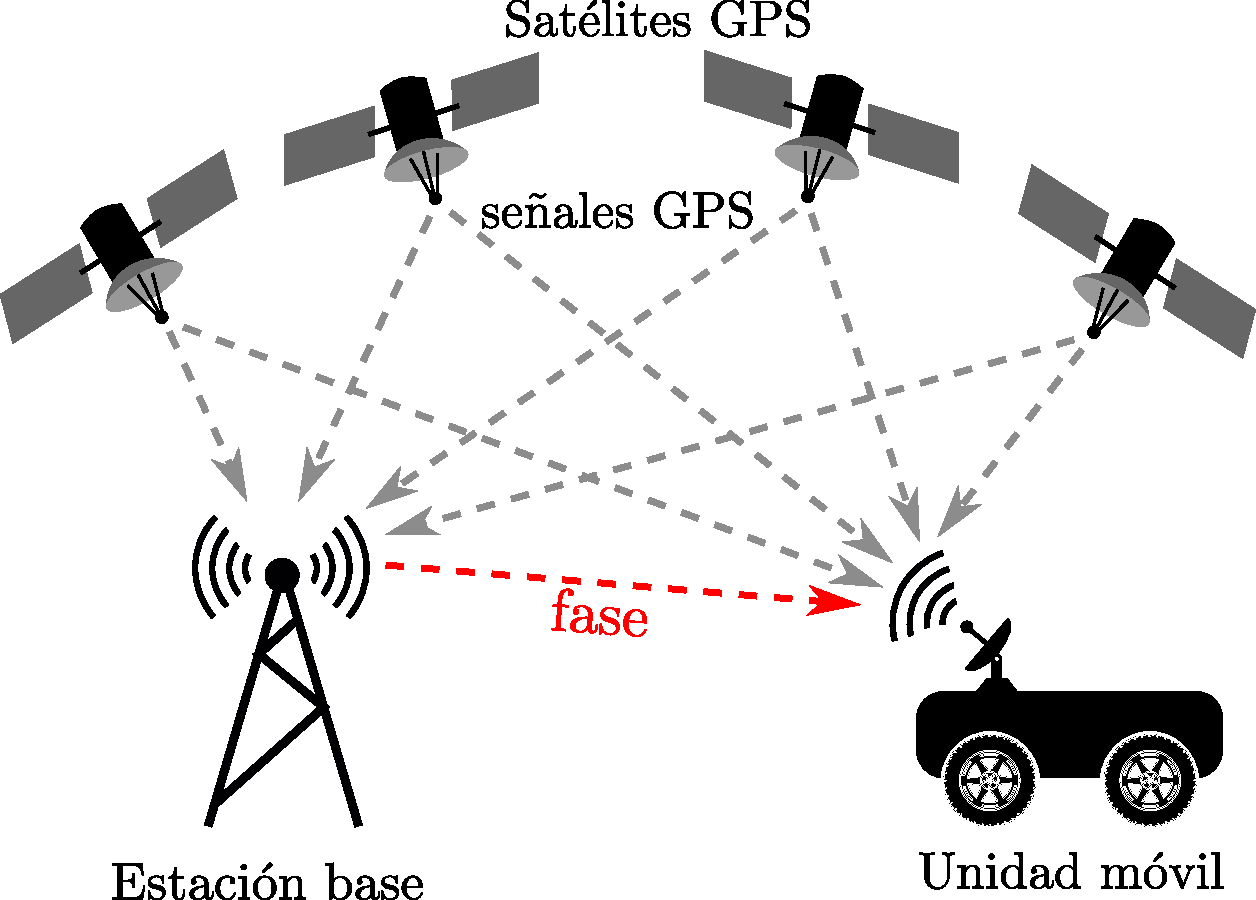
\includegraphics[width=0.3\columnwidth]{gps_rtk_system.pdf}
    \end{center}

\end{frame}